
\documentclass[a4paper,final,12pt]{article}
%%%%%%%%%%%%%%%%%%%%%%%%%%%%%%%%%%%%%%%%%%%%%%%%%%%%%%%%%%%%%%%%%%%%%%%%%%%%%%%%%%%%%%%%%%%%%%%%%%%%%%%%%%%%%%%%%%%%%%%%%%%%%%%%%%%%%%%%%%%%%%%%%%%%%%%%%%%%%%%%%%%%%%%%%%%%%%%%%%%%%%%%%%%%%%%%%%%%%%%%%%%%%%%%%%%%%%%%%%%%%%%%%%%%%%%%%%%%%%%%%%%%%%%%%%%%
\usepackage{graphicx,hyperref,mathpple,amsmath,exscale,setspace,xcolor}
\usepackage[left=20mm,right=20mm,top=20mm,bottom=20mm]{geometry}
\usepackage{pdflscape,showkeys,changepage}
\usepackage[TABBOTCAP]{subfigure}
\usepackage[round]{natbib}

\setcounter{MaxMatrixCols}{10}
%TCIDATA{OutputFilter=LATEX.DLL}
%TCIDATA{Version=5.50.0.2953}
%TCIDATA{<META NAME="SaveForMode" CONTENT="2">}
%TCIDATA{BibliographyScheme=BibTeX}
%TCIDATA{Created=Wednesday, May 03, 2023 13:45:06}
%TCIDATA{LastRevised=Monday, January 15, 2024 21:40:43}
%TCIDATA{<META NAME="GraphicsSave" CONTENT="32">}
%TCIDATA{<META NAME="DocumentShell" CONTENT="Standard LaTeX\Blank - Standard LaTeX Article">}
%TCIDATA{CSTFile=40 LaTeX article.cst}

\AtBeginDocument{
\let\oldref\ref\renewcommand{\ref}[1]{(\oldref{#1})}
\newcommand{\bsq}{\begin{subequations}}\newcommand{\esq}{\end{subequations}}
\newcommand{\bls}{\begin{landscape}}\newcommand{\els}{\end{landscape}}
\renewcommand\showkeyslabelformat[1]{{\parbox[t]{\marginparwidth}{\raggedright\footnotesize\url{#1}}}}
\newcommand{\intxt}[1]{\intertext{#1}}\newcommand{\BAW}[1]{\begin{adjustwidth}{-#1mm}{-5mm}}\newcommand{\EAW}{\end{adjustwidth}}
\newcommand{\vsp}[1]{\vspace*{#1mm}}\newcommand{\hsp}[1]{\hspace*{#1mm}}  }
\renewcommand\section{\@startsection{section}{1}{\z@}{-2.5ex \@plus -1ex \@minus -.2ex}{0.01ex \@plus.2ex}{\Large\bfseries}}
\renewcommand\subsection{\@startsection{subsection}{1}{\z@}{-1.5ex \@plus -1ex \@minus -.2ex}{0.01ex \@plus.2ex}{\large\bfseries}}
\makeatletter
\renewcommand*{\@fnsymbol}[1]{\ensuremath{\ifcase#1\or *\or
    \#\or \star\or \bowtie\or \star\star\or \ddagger\ddagger \else\@ctrerr\fi}}
\makeatother
\allowdisplaybreaks
\IfFileExists{C:/swp55/TCITeX/TeX/LaTeX/SWmacros/tcilatex.tex}{\input{tcilatex}}{}
\graphicspath{{./graphics/}{../graphics/}{../../graphics/}}
\definecolor{myred}{rgb}{.50,.10,.10}
\definecolor{mygrn}{rgb}{.10,.35,.10}
\definecolor{myblu}{rgb}{.10,.10,.35}
\hypersetup{colorlinks,citecolor=myblu,filecolor=mygrn,linkcolor=myred,urlcolor=mygrn,breaklinks=true}
\setstretch{1.2345}
\setlength{\parskip}{7pt}

\begin{document}


\section{Clark87}

The Clark (1987) Unobserved Component (UC) model is a generalisation of the
HP--Filter (a local linear trend model) that can be expressed in State Space
Form (SSF) as:\bsq\label{clark0}%
\begin{align}
y_{t}& =y_{t}^{\ast }+\tilde{y}_{t} \\
\Delta y_{t}^{\ast }& =g_{t-1}+\sigma _{1}\varepsilon _{1t} \\
\Delta g_{t}& =\sigma _{2}\varepsilon _{2t} \\
a(L)\tilde{y}_{t}& =\sigma _{3}\varepsilon _{3t},
\end{align}%
\esq where $y_{t}$ is (100 times) the log of GDP, and the shocks $\left\{
\varepsilon _{it}\right\} _{i=1}^{3}$ are mutually uncorrelated $i.i.d.$ $%
N(0,1)$, with standard deviations $\left\{ \sigma _{i}\right\} _{i=1}^{3}$,
and $a(L)$ is a lag polynomial commonly assumed to be a stable AR(2), ie., $%
a(L)=(1-a_{1}L-a_{2}L^{2})$, with the roots of $a(L)$ being outside the unit
circle. The cycle $\tilde{y}_{t}$ is allowed to be serially correlated.
There are 3 shocks in the model.

The `\emph{numbered} \emph{shock}' to `\emph{named shock}' mapping is:%
\begin{equation}
\begin{bmatrix}
\varepsilon _{1t} \\ 
\varepsilon _{2t} \\ 
\varepsilon _{3t}%
\end{bmatrix}%
=%
\begin{bmatrix}
\varepsilon _{t}^{y^{\ast }} \\ 
\varepsilon _{t}^{g} \\ 
\varepsilon _{t}^{\tilde{y}}%
\end{bmatrix}%
,
\end{equation}%
where $\varepsilon _{t}^{y^{\ast }}$, $\varepsilon _{t}^{g}$, and $%
\varepsilon _{t}^{\tilde{y}}$ are the trend (permanent), trend growth and
cycle shocks, respectively.

\section{Shock recovery}

\subsection{State Space Models with lagged states}

Kurz's (2018) SSM has the following general from:\bsq\label{SSM}%
\begin{align}
\mathsf{Measurement}& :\quad Z_{t}=D_{1}X_{t}+D_{2}X_{t-1}+R\varepsilon _{t}
\label{ssm1} \\
\mathsf{State}& :\quad X_{t}=AX_{t-1}+C\varepsilon _{t},  \label{ssm2}
\end{align}%
\esq where $\varepsilon _{t}\sim MN(0_{m},I_{m})$, $D_{1},D_{2},A,R$ are $C$
are conformable system matrices, $Z_{t}$ the observed variable and $X_{t}$
the latent state variable, and $m$ is the number of shocks $\left\{
\varepsilon _{it}\right\} _{i=1}^{m}$.

\subsection{Clark87 in `\emph{shock recovery}' SSF}

To assess shock recovery, write the model in \ref{clark0} in `\emph{shock
recovery}' SSF by collecting all observable variables in $Z_{t}$ and all
shocks (and other latent state variables)\ in $X_{t}$. Differencing $y_{t}$
and $y_{t}^{c}$ twice, and re-arranging the relations in \ref{clark0}\ then
yields:%
\begin{align}
\Delta ^{2}y_{t}& =\Delta ^{2}y_{t}^{\ast }+\Delta ^{2}\tilde{y}_{t}  \notag
\\
& =\sigma _{1}\Delta \varepsilon _{1t}+\Delta g_{t-1}+\Delta ^{2}\tilde{y}%
_{t}  \notag \\
& =\sigma _{1}\Delta \varepsilon _{1t}+\sigma _{2}\varepsilon
_{2t-1}+a(L)^{-1}\sigma _{3}\Delta ^{2}\varepsilon _{3t}  \notag \\
\Leftrightarrow a(L)\Delta ^{2}y_{t}& =\sigma _{1}a(L)\Delta \varepsilon
_{1t}+\sigma _{2}a(L)\varepsilon _{2t-1}+\sigma _{3}\Delta ^{2}\varepsilon
_{3t}  \label{clark1}
\end{align}%
where $a(L)\Delta ^{2}y_{t}$ is the only observed variable. Re-writing \ref%
{clark1} in more convenient form for the SSF yields:%
\begin{equation}
\begin{split}
\underbrace{a(L)\Delta ^{2}y_{t}}_{Z_{t}}& =a(L)\sigma _{1}\Delta
\varepsilon _{1t}+a(L)\sigma _{2}\varepsilon _{2t-1}+\sigma _{3}\Delta
^{2}\varepsilon _{3t} \\[-5.5mm]
& =\sigma _{1}\Delta \varepsilon _{1t}-a_{1}\sigma _{1}\Delta \varepsilon
_{1t-1}-a_{2}\sigma _{1}\Delta \varepsilon _{1t-2}+\sigma _{2}\varepsilon
_{2t-1}-a_{1}\sigma _{2}\varepsilon _{2t-2} \\
& -\ a_{2}\sigma _{2}\varepsilon _{2t-3}+\sigma _{3}\Delta \varepsilon
_{3t}-\sigma _{3}\Delta \varepsilon _{3t-1}.
\end{split}
\label{Z}
\end{equation}

The Measurement and State equations of the `\emph{shock recovery}' SSF
corresponding to the relations in \ref{Z} are then given by:\bsq\label{K0SSM}%
\begin{eqnarray}
\mathsf{Measurement}:\quad Z_{t} &=&D_{1}X_{t}+D_{2}X_{t-1}+R\varepsilon _{t}
\\[-17mm]
Z_{t} &=&\underbrace{%
\begin{bmatrix}
0 & 0 & 0 & \sigma _{1} & -a_{1}\sigma _{1} & 0 & 0 & \sigma _{3}%
\end{bmatrix}%
}_{D_{1}}\underbrace{%
\begin{bmatrix}
\varepsilon _{1t} \\ 
\varepsilon _{2t} \\ 
\varepsilon _{3t} \\ 
\Delta \varepsilon _{1t} \\ 
\Delta \varepsilon _{1t-1} \\ 
\varepsilon _{2t-1} \\ 
\varepsilon _{2t-2} \\ 
\Delta \varepsilon _{3t}%
\end{bmatrix}%
}_{X_{t}} \\[-17mm]
&+&\underbrace{%
\begin{bmatrix}
0 & \sigma _{2} & 0 & 0 & -a_{2}\sigma _{1} & -a_{1}\sigma _{2} & 
-a_{2}\sigma _{2} & -\sigma _{3}%
\end{bmatrix}%
}_{D_{2}}\underbrace{%
\begin{bmatrix}
\varepsilon _{1t-1} \\ 
\varepsilon _{2t-1} \\ 
\varepsilon _{3t-1} \\ 
\Delta \varepsilon _{1t-1} \\ 
\Delta \varepsilon _{1t-2} \\ 
\varepsilon _{2t-2} \\ 
\varepsilon _{2t-3} \\ 
\Delta \varepsilon _{3t-1}%
\end{bmatrix}%
}_{X_{t-1}}+\underbrace{%
\begin{bmatrix}
0 & 0 & 0%
\end{bmatrix}%
}_{R}\underbrace{%
\begin{bmatrix}
\varepsilon _{1t} \\ 
\varepsilon _{2t} \\ 
\varepsilon _{3t}%
\end{bmatrix}%
}_{\varepsilon _{t}}  \notag
\end{eqnarray}

\vspace*{-12mm}

\begin{align}
\mathsf{State}:\quad X_{t}& =AX_{t-1}+C\varepsilon _{t} \\
\underbrace{%
\begin{bmatrix}
\varepsilon _{1t} \\ 
\varepsilon _{2t} \\ 
\varepsilon _{3t} \\ 
\Delta \varepsilon _{1t} \\ 
\Delta \varepsilon _{1t-1} \\ 
\varepsilon _{2t-1} \\ 
\varepsilon _{2t-2} \\ 
\Delta \varepsilon _{3t}%
\end{bmatrix}%
}_{X_{t}}& =\underbrace{%
\begin{bmatrix}
0 & 0 & 0 & 0 & 0 & 0 & 0 & 0 \\ 
0 & 0 & 0 & 0 & 0 & 0 & 0 & 0 \\ 
0 & 0 & 0 & 0 & 0 & 0 & 0 & 0 \\ 
-1 & 0 & 0 & 0 & 0 & 0 & 0 & 0 \\ 
0 & 0 & 0 & 1 & 0 & 0 & 0 & 0 \\ 
0 & 1 & 0 & 0 & 0 & 0 & 0 & 0 \\ 
0 & 0 & 0 & 0 & 0 & 1 & 0 & 0 \\ 
0 & 0 & -1 & 0 & 0 & 0 & 0 & 0%
\end{bmatrix}%
}_{A}\underbrace{%
\begin{bmatrix}
\varepsilon _{1t-1} \\ 
\varepsilon _{2t-1} \\ 
\varepsilon _{3t-1} \\ 
\Delta \varepsilon _{1t-1} \\ 
\Delta \varepsilon _{1t-2} \\ 
\varepsilon _{2t-2} \\ 
\varepsilon _{2t-3} \\ 
\Delta \varepsilon _{3t-1}%
\end{bmatrix}%
}_{X_{t-1}}+\underbrace{%
\begin{bmatrix}
1 & 0 & 0 \\ 
0 & 1 & 0 \\ 
0 & 0 & 1 \\ 
1 & 0 & 0 \\ 
0 & 0 & 0 \\ 
0 & 0 & 0 \\ 
0 & 0 & 0 \\ 
0 & 0 & 1%
\end{bmatrix}%
}_{C}\underbrace{%
\begin{bmatrix}
\varepsilon _{1t} \\ 
\varepsilon _{2t} \\ 
\varepsilon _{3t}%
\end{bmatrix}%
}_{\varepsilon _{t}}.
\end{align}%
\esq

\subsection{Shock recovery}

The diagonal of the steady-state variance/covariance matrix of the smoothed
and filtered states $X_{t}$ denoted by $P_{t|T}^{\ast }$ and $P_{t|t}^{\ast
} $, respectively, are:%
\begin{equation}
\begin{tabular}{ccccc}
\hline
Shocks &  & $P_{t|T}^{\ast }$ &  & $P_{t|t}^{\ast }$ \\ \hline
$\varepsilon _{1t}$ &  & $0.5469$ &  & $0.5989$ \\ 
$\varepsilon _{2t}$ &  & $0.9870$ &  & $1.0000$ \\ 
$\varepsilon _{3t}$ &  & $0.4661$ &  & $0.5153$ \\ \hline
\end{tabular}%
~,  \label{Pstar}
\end{equation}%
indicating that the trend growth shock $\varepsilon _{2t}=\varepsilon
_{t}^{g}$ cannot be recovered ($P^{\ast }\approx 1$), while the cycle shock $%
\varepsilon _{3t}=\varepsilon _{t}^{\tilde{y}}$ and the trend shock $%
\varepsilon _{1t}=\varepsilon _{t}^{y^{\ast }}$ have $P^{\ast }\approx 0.5$,
suggesting that there are recovery difficulties. Note that $P_{t|t}^{\ast
}=1 $ implies that Kalman filtered estimates of $\varepsilon _{2t}$ are 
\emph{exactly} zero for all $t$. This can be seen from the entries on the
left hand side of \ref{KFS} which shows filtered estimates of shocks
(smoothed estimates are shown on the right hand side).%
\begin{equation}
\begin{tabular}{rcrcrrr}
\hline
\multicolumn{3}{c}{Filtered} & ~~ & \multicolumn{3}{c}{Smoothed$\ $} \\ 
$E_{t}\varepsilon _{1t}\ \ $ & $E_{t}\varepsilon _{2t}$ & $E_{t}\varepsilon
_{3t}\ \ $ & ~~ & $E_{T}\varepsilon _{1t}\ \ $ & $E_{T}\varepsilon _{2t}\ \ $
& $E_{T}\varepsilon _{3t}\ \ $ \\ \hline
$-0.7088$ & $0$ & $-0.7792$ &  & $0.3098$ & $-0.0160$ & $0.0344$ \\ 
$-0.8039$ & $0$ & $-0.8837$ &  & $-0.5269$ & $0.0043$ & $-0.5442$ \\ 
$-0.2554$ & $0$ & $-0.2808$ &  & $-0.1336$ & $0.0094$ & $0.1118$ \\ 
$0.0179$ & $0$ & $0.0196$ &  & $0.6757$ & $-0.0166$ & $0.4942$ \\ 
$-0.5488$ & $0$ & $-0.6032$ &  & $-0.2535$ & $-0.0068$ & $-0.4492$ \\ 
$-0.3244$ & $0$ & $-0.3566$ &  & $-0.3713$ & $0.0075$ & $-0.2660$ \\ 
$0.1304$ & $0$ & $0.1434$ &  & $0.2703$ & $-0.0029$ & $0.3115$ \\ 
$-0.2821$ & $0$ & $-0.3101$ &  & $-0.6689$ & $0.0228$ & $0.0549$ \\ \hline
\end{tabular}%
~.  \label{KFS}
\end{equation}%
In \autoref{fig:1}, simulated states and corresponding Kalman smoothed
estimates are plotted for the shocks of interest.

The correlation between the true (simulated) and estimated Kalman smoothed
shocks can be analyzed by simply computing $\mathrm{Corr}(X_{t},\hat{X}%
_{t|T})$, where $X_{t}=%
\begin{bmatrix}
\varepsilon _{1t} & \varepsilon _{2t} & \varepsilon _{3t}%
\end{bmatrix}%
^{\prime }$ and $\hat{X}_{t|T}=E_{T}X_{t}=E_{T}%
\begin{bmatrix}
\varepsilon _{1t} & \varepsilon _{2t} & \varepsilon _{2t-1}%
\end{bmatrix}%
^{\prime }$, which yields:%
\begin{equation}
\begin{tabular}{ccc}
\hline
Shocks &  & $\mathrm{Corr}(X_{t},\hat{X}_{t|T})$ \\ \hline
$\varepsilon _{1t}$ &  & $0.6736$ \\ 
$\varepsilon _{2t}$ &  & $0.1184$ \\ 
$\varepsilon _{3t}$ &  & $0.7304$ \\ \hline
\end{tabular}%
~.  \label{Corr}
\end{equation}%
From \ref{Corr} one can see that the estimated $\varepsilon _{1t}$ and $%
\varepsilon _{3t}$ shocks are rather `\emph{weakly}' correlated with the
true values, $0.6736$ and $0.7304$, respectively. The estimated $\varepsilon
_{2t}$ shock is nearly uncorrelated ($0.1184$) with the true value.\ These
facts can also be seen from \autoref{fig:1} below.

\begin{figure}[h!]
  \centering
  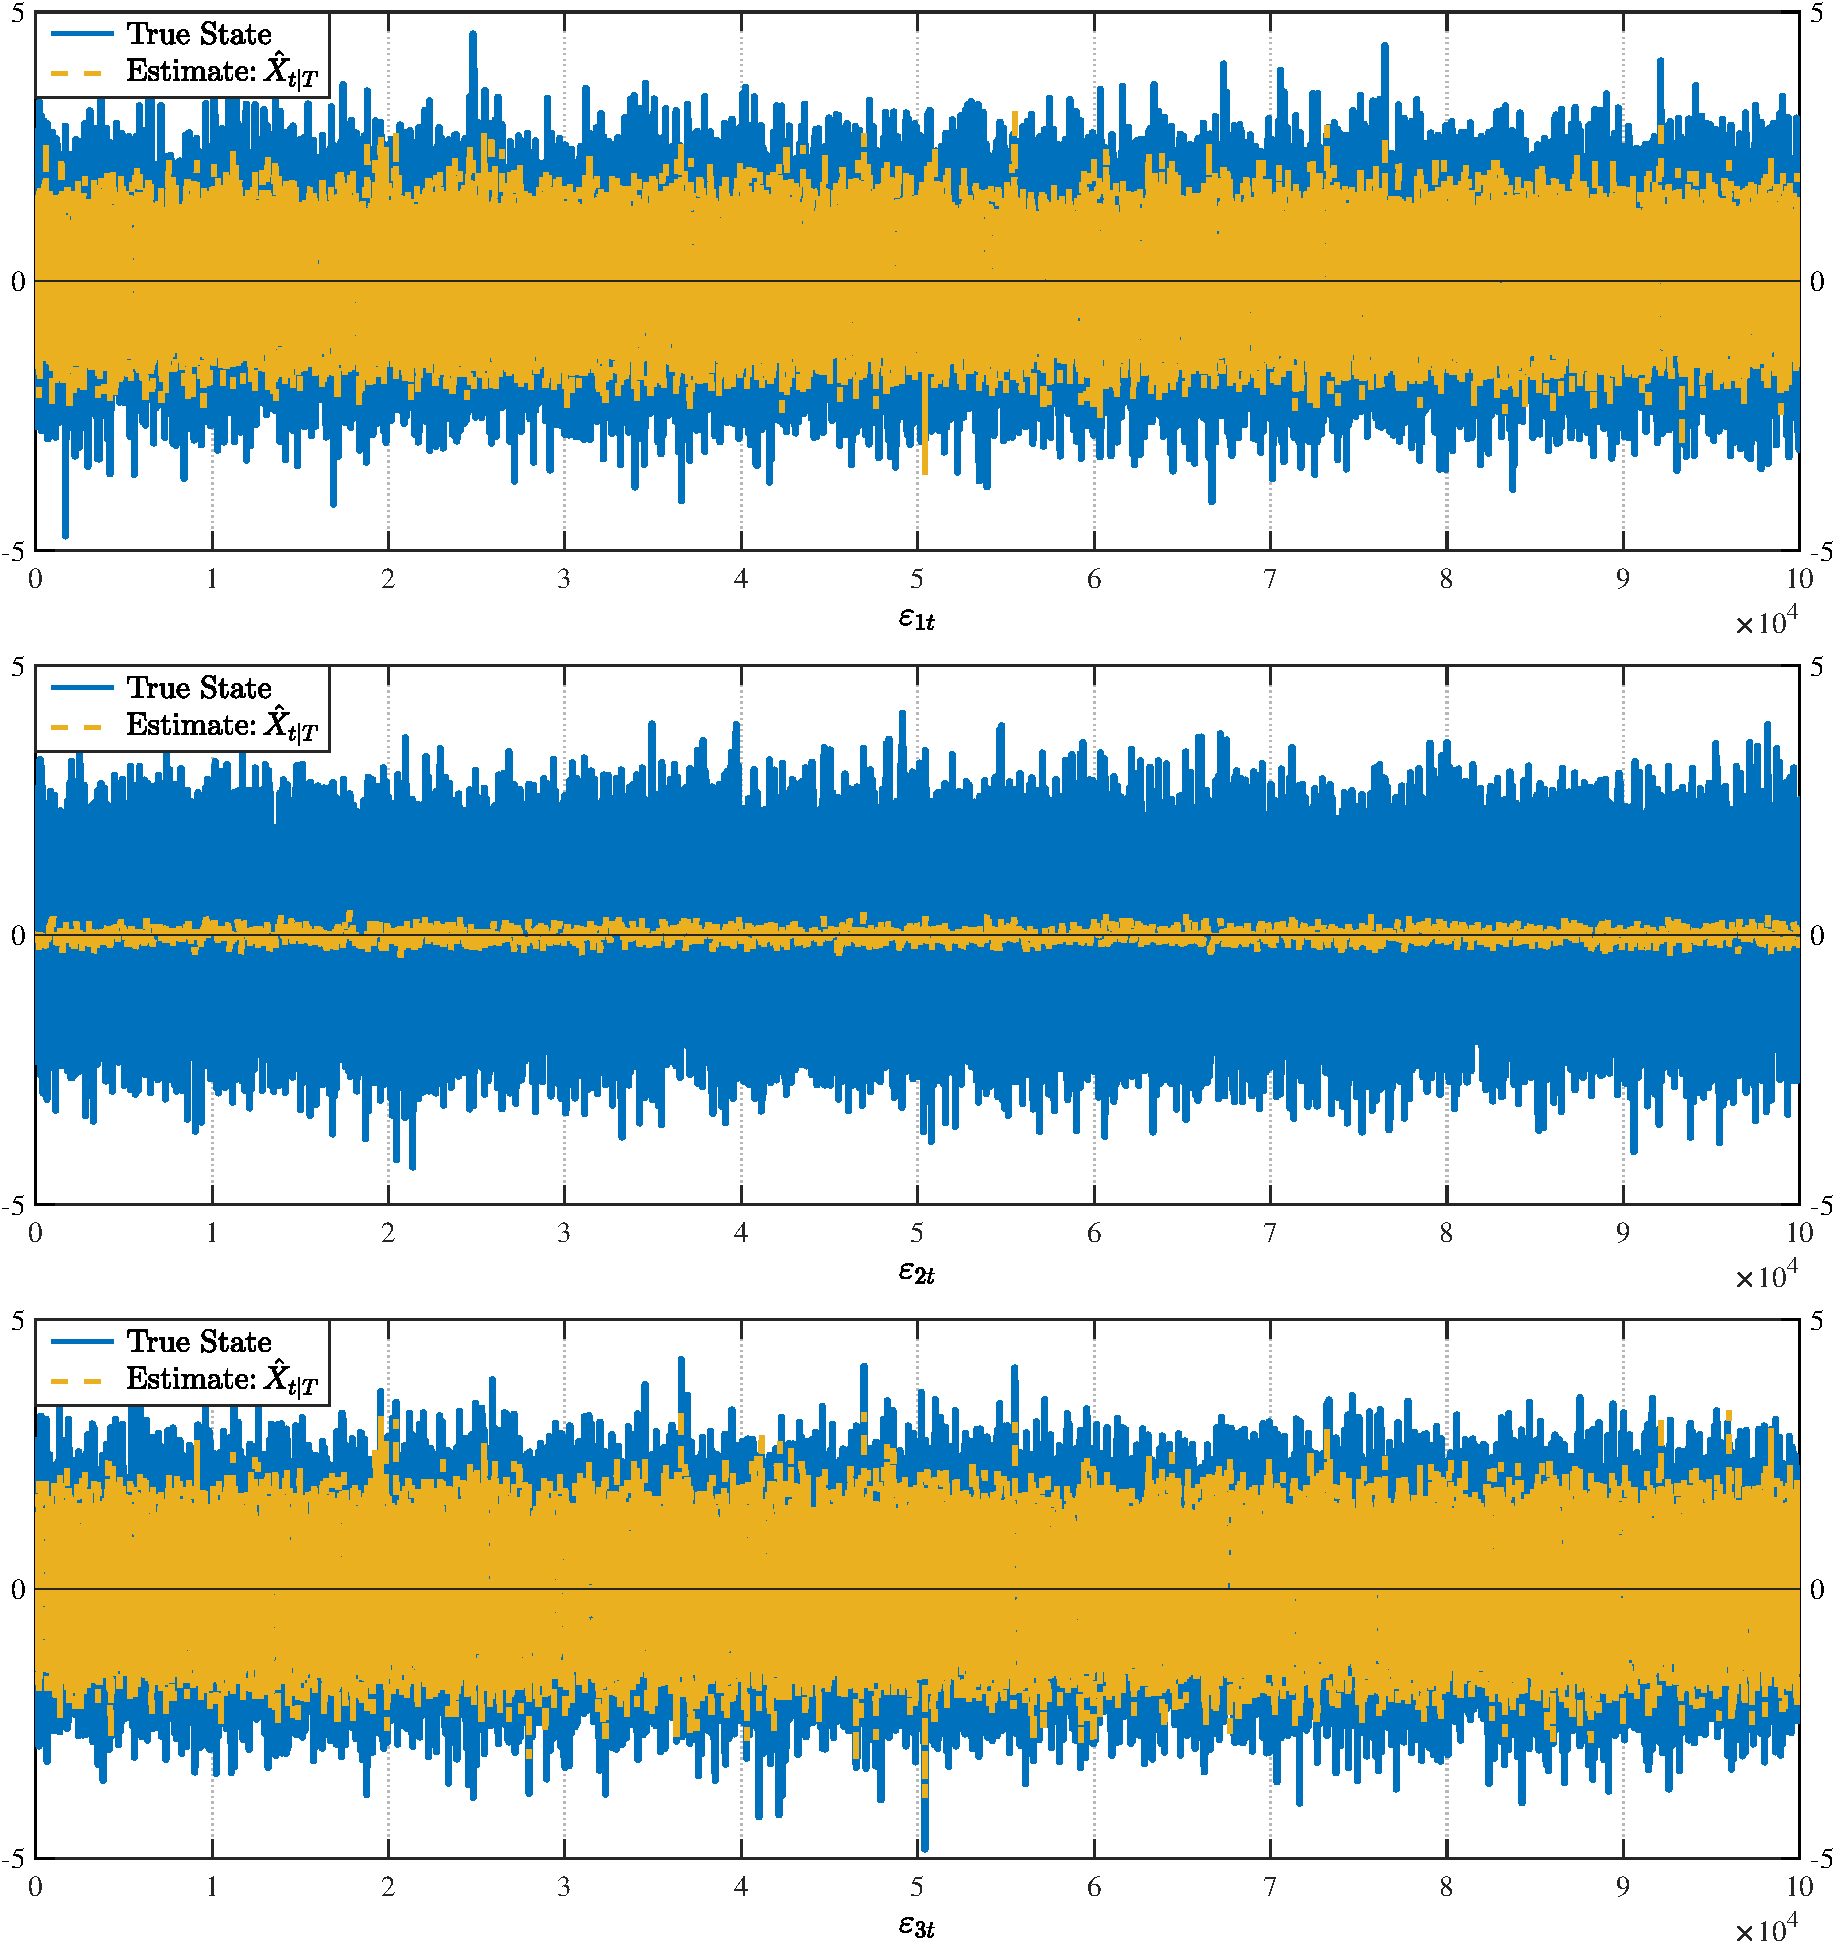
\includegraphics[width=1\textwidth,trim={0 0 0
  0},clip,angle=00]{Clark87_plots_KS.pdf}
  \caption{Comparison of true shocks and Kalman Smoothed estimates $\protect%
  \varepsilon _{t|T}$.}
  \label{fig:1}
\end{figure}

\subsection{Shock Identities}

As was the case for the HP-Filter, the Kalman filtered estimates of the
trend and cycle shocks $\varepsilon _{1t}$ and $\varepsilon _{3t}$ are
linked by the (filter) identity:%
\begin{equation}
E_{t}\varepsilon _{1t}=0.909694E_{t}\varepsilon _{3t}.  \label{KF}
\end{equation}%
Kalman smoothed estimates give the following \emph{dynamic} identities:%
\begin{equation}
\Delta ^{2}E_{T}\varepsilon _{2t}=-0.038486\Delta E_{T}\varepsilon _{1t},
\label{KS1}
\end{equation}%
and also:%
\begin{align}
\Delta ^{2}E_{T}\varepsilon _{3t}& =-1.935746\Delta E_{T}\varepsilon
_{1t-1}+1.659427E_{T}\varepsilon _{3t-1}-1.760937E_{T}\varepsilon _{3t-2}
\label{KS2a} \\
\Delta ^{2}E_{T}\varepsilon _{3t}& =50.297162\Delta E_{T}\varepsilon
_{2t-1}+1.659427E_{T}\varepsilon _{3t-1}-1.760937E_{T}\varepsilon _{3t-2}.
\label{KS2b}
\end{align}

The contemporaneous correlations of the shocks from the Kalman filtered and
smoothed estimates are, respectively: 
\begin{equation*}
\begin{tabular}{lccr}
\multicolumn{4}{c}{$\mathrm{Corr}(\hat{X}_{t|t},\hat{X}_{t|t})$} \\ \hline
Shocks & {$\varepsilon _{1t}$} & {$\varepsilon _{2t}$} & $\varepsilon _{3t}$
\\ \hline
\multicolumn{1}{c}{$\varepsilon _{1t}$} & \multicolumn{1}{r}{$1.0000$} & $%
\mathrm{NaN}$ & $1.0000$ \\ 
\multicolumn{1}{c}{$\varepsilon _{2t}$} & $\mathrm{NaN}$ & $\mathrm{NaN}$ & 
\multicolumn{1}{c}{$\mathrm{NaN}$} \\ 
\multicolumn{1}{c}{$\varepsilon _{3t}$} & \multicolumn{1}{r}{$1.0000$} & $%
\mathrm{NaN}$ & $1.0000$ \\ \hline
\end{tabular}%
\text{ \ \ \ \ and \ \ \ \ }%
\begin{tabular}{lccc}
\multicolumn{4}{c}{$\mathrm{Corr}(\hat{X}_{t|T},\hat{X}_{t|T})$} \\ \hline
Shocks & {$\varepsilon _{1t}$} & {$\varepsilon _{2t}$} & $\varepsilon _{3t}$
\\ \hline
\multicolumn{1}{c}{$\varepsilon _{1t}$} & \multicolumn{1}{r}{$1.0000$} & 
\multicolumn{1}{r}{$-0.1104$} & \multicolumn{1}{r}{$1.0000$} \\ 
\multicolumn{1}{c}{$\varepsilon _{2t}$} & $-0.1104$ & \multicolumn{1}{r}{$%
1.0000$} & $-0.1446$ \\ 
\multicolumn{1}{c}{$\varepsilon _{3t}$} & \multicolumn{1}{r}{$0.8403$} & 
\multicolumn{1}{r}{$-0.1446$} & \multicolumn{1}{r}{$1.0000$} \\ \hline
\end{tabular}%
~\text{.}
\end{equation*}%
Note that the $\left\{ {\varepsilon _{it}}\right\} _{i=1}^{3}${\ }were
generated as mutually uncorrelated $i.i.d.$ $N(0,1)$ processes, while their `%
\emph{large sample}' estimates are correlated. The code\ $\mathtt{Clark87.m}$
replicates the output summarized here. \ 

\subsection{Maximum Likelihood estimation}

The (standard)\ SSF\ for ML\ estimation for the model in \ref{clark0} is:%
\begin{align}
y_{t}& =%
\begin{bmatrix}
1 & 0 & 1 & 0%
\end{bmatrix}%
\begin{bmatrix}
y_{t}^{\ast } \\ 
g_{t} \\ 
\tilde{y}_{t} \\ 
\tilde{y}_{t-1}%
\end{bmatrix}%
+0\varepsilon _{t} \\[4mm]
\begin{bmatrix}
y_{t}^{\ast } \\ 
g_{t} \\ 
\tilde{y}_{t} \\ 
\tilde{y}_{t-1}%
\end{bmatrix}%
& =%
\begin{bmatrix}
1 & 1 & 0 & 0 \\ 
0 & 1 & 0 & 0 \\ 
0 & 0 & a_{1} & a_{2} \\ 
0 & 0 & 1 & 0%
\end{bmatrix}%
\begin{bmatrix}
y_{t-1}^{\ast } \\ 
g_{t-1} \\ 
\tilde{y}_{t-1} \\ 
\tilde{y}_{t-2}%
\end{bmatrix}%
+%
\begin{bmatrix}
\sigma _{1} & 0 & 0 \\ 
0 & \sigma _{2} & 0 \\ 
0 & 0 & \sigma _{3} \\ 
0 & 0 & 0%
\end{bmatrix}%
\begin{bmatrix}
\varepsilon _{1t} \\ 
\varepsilon _{2t} \\ 
\varepsilon _{3t}%
\end{bmatrix}%
.
\end{align}%
Below are estimates and plots of Clark's 87 model fitted to U.S. GDP\ data
from $1947$:Q2 to $2019$:Q4. 
\begin{table}[h!]
\centering
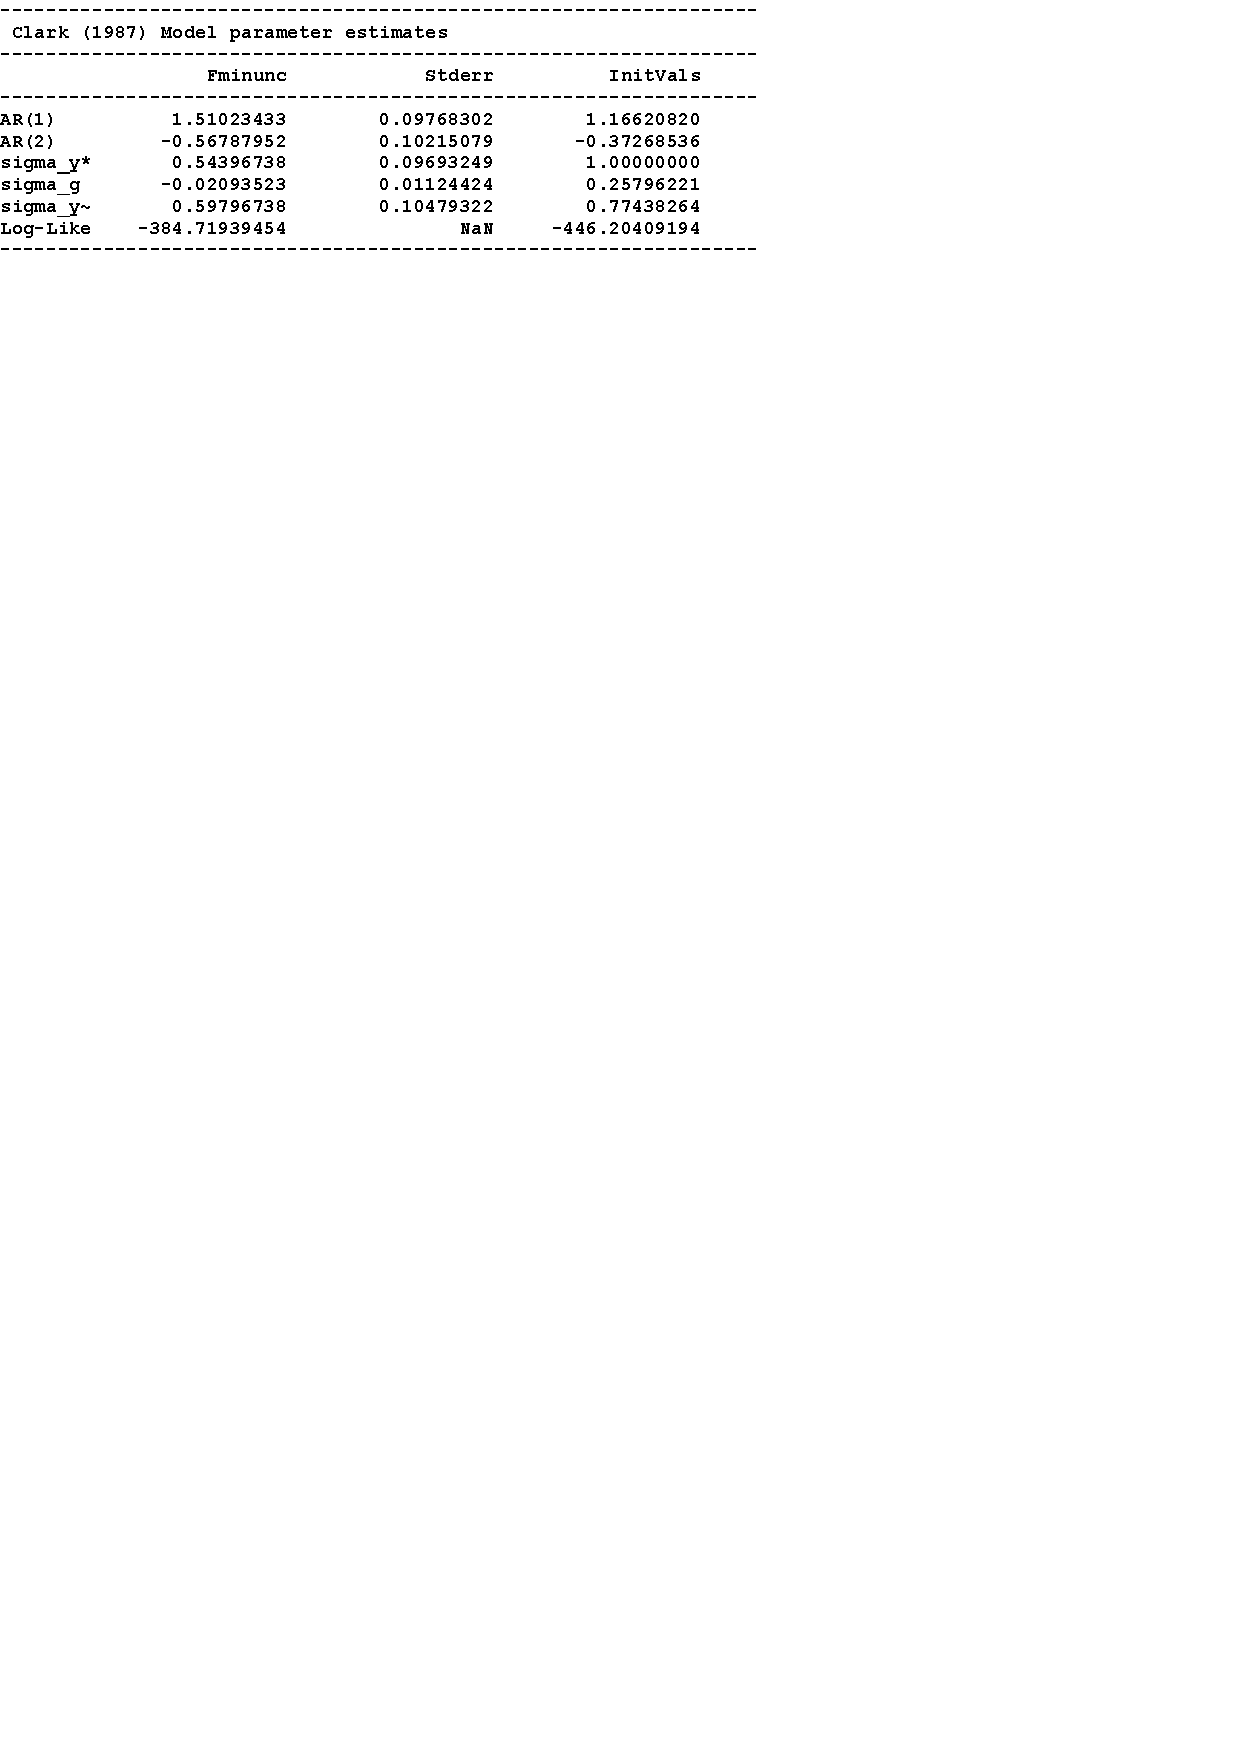
\includegraphics[width=.75\textwidth,trim={0 0 0 25},clip]{Clark_MLE.pdf} 
\vspace*{-2.5mm}
\caption{Clark (1987) model MLE parameter estimates for the U.S. from $1947$%
:Q2 to $2019$:Q4.}
\label{tab:MLE}
\end{table}

\begin{figure}[p!]
\centering
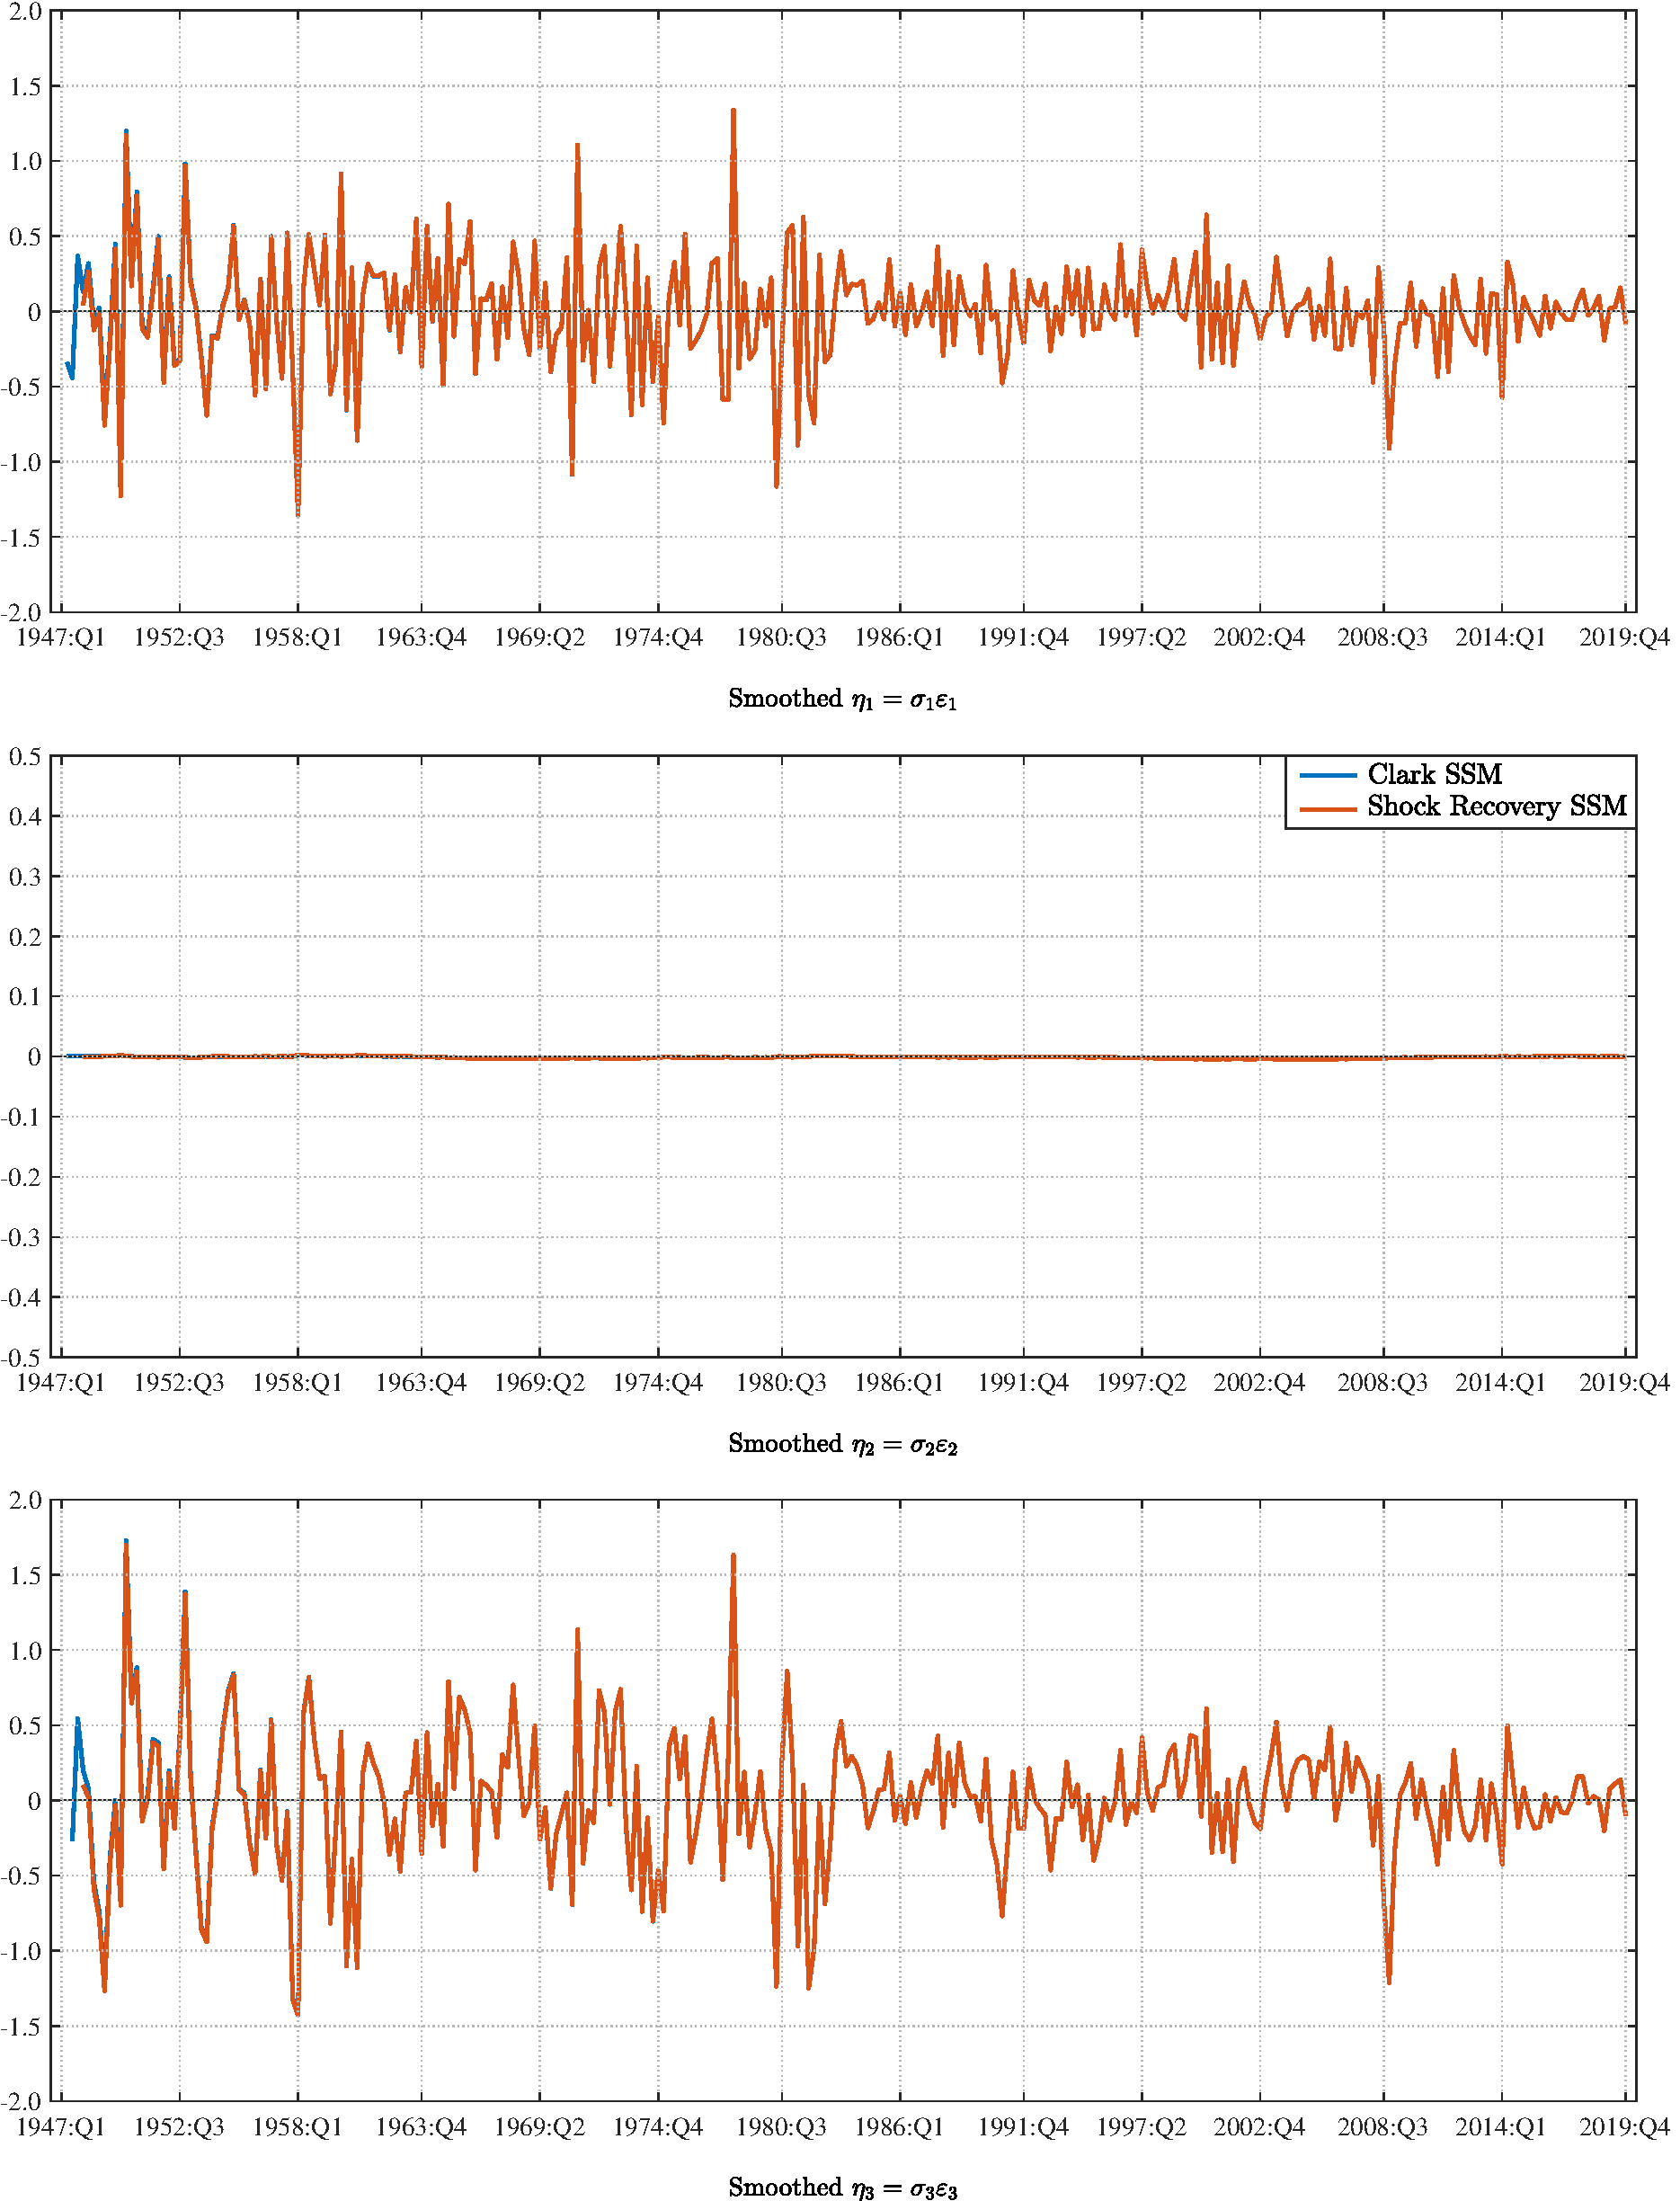
\includegraphics[angle=00, width=1\textwidth,trim={0 0 0
0},clip]{Clark_SSM_Smoothed.pdf} \vspace*{-2.5mm}
\caption{Smoother estimates of scaled shocks $\protect\eta_{it} = \protect%
\sigma_i\protect\varepsilon_{it}, \forall i=1,2,3$.}
\label{fig:KS}
\end{figure}

\begin{figure}[p!]
\centering
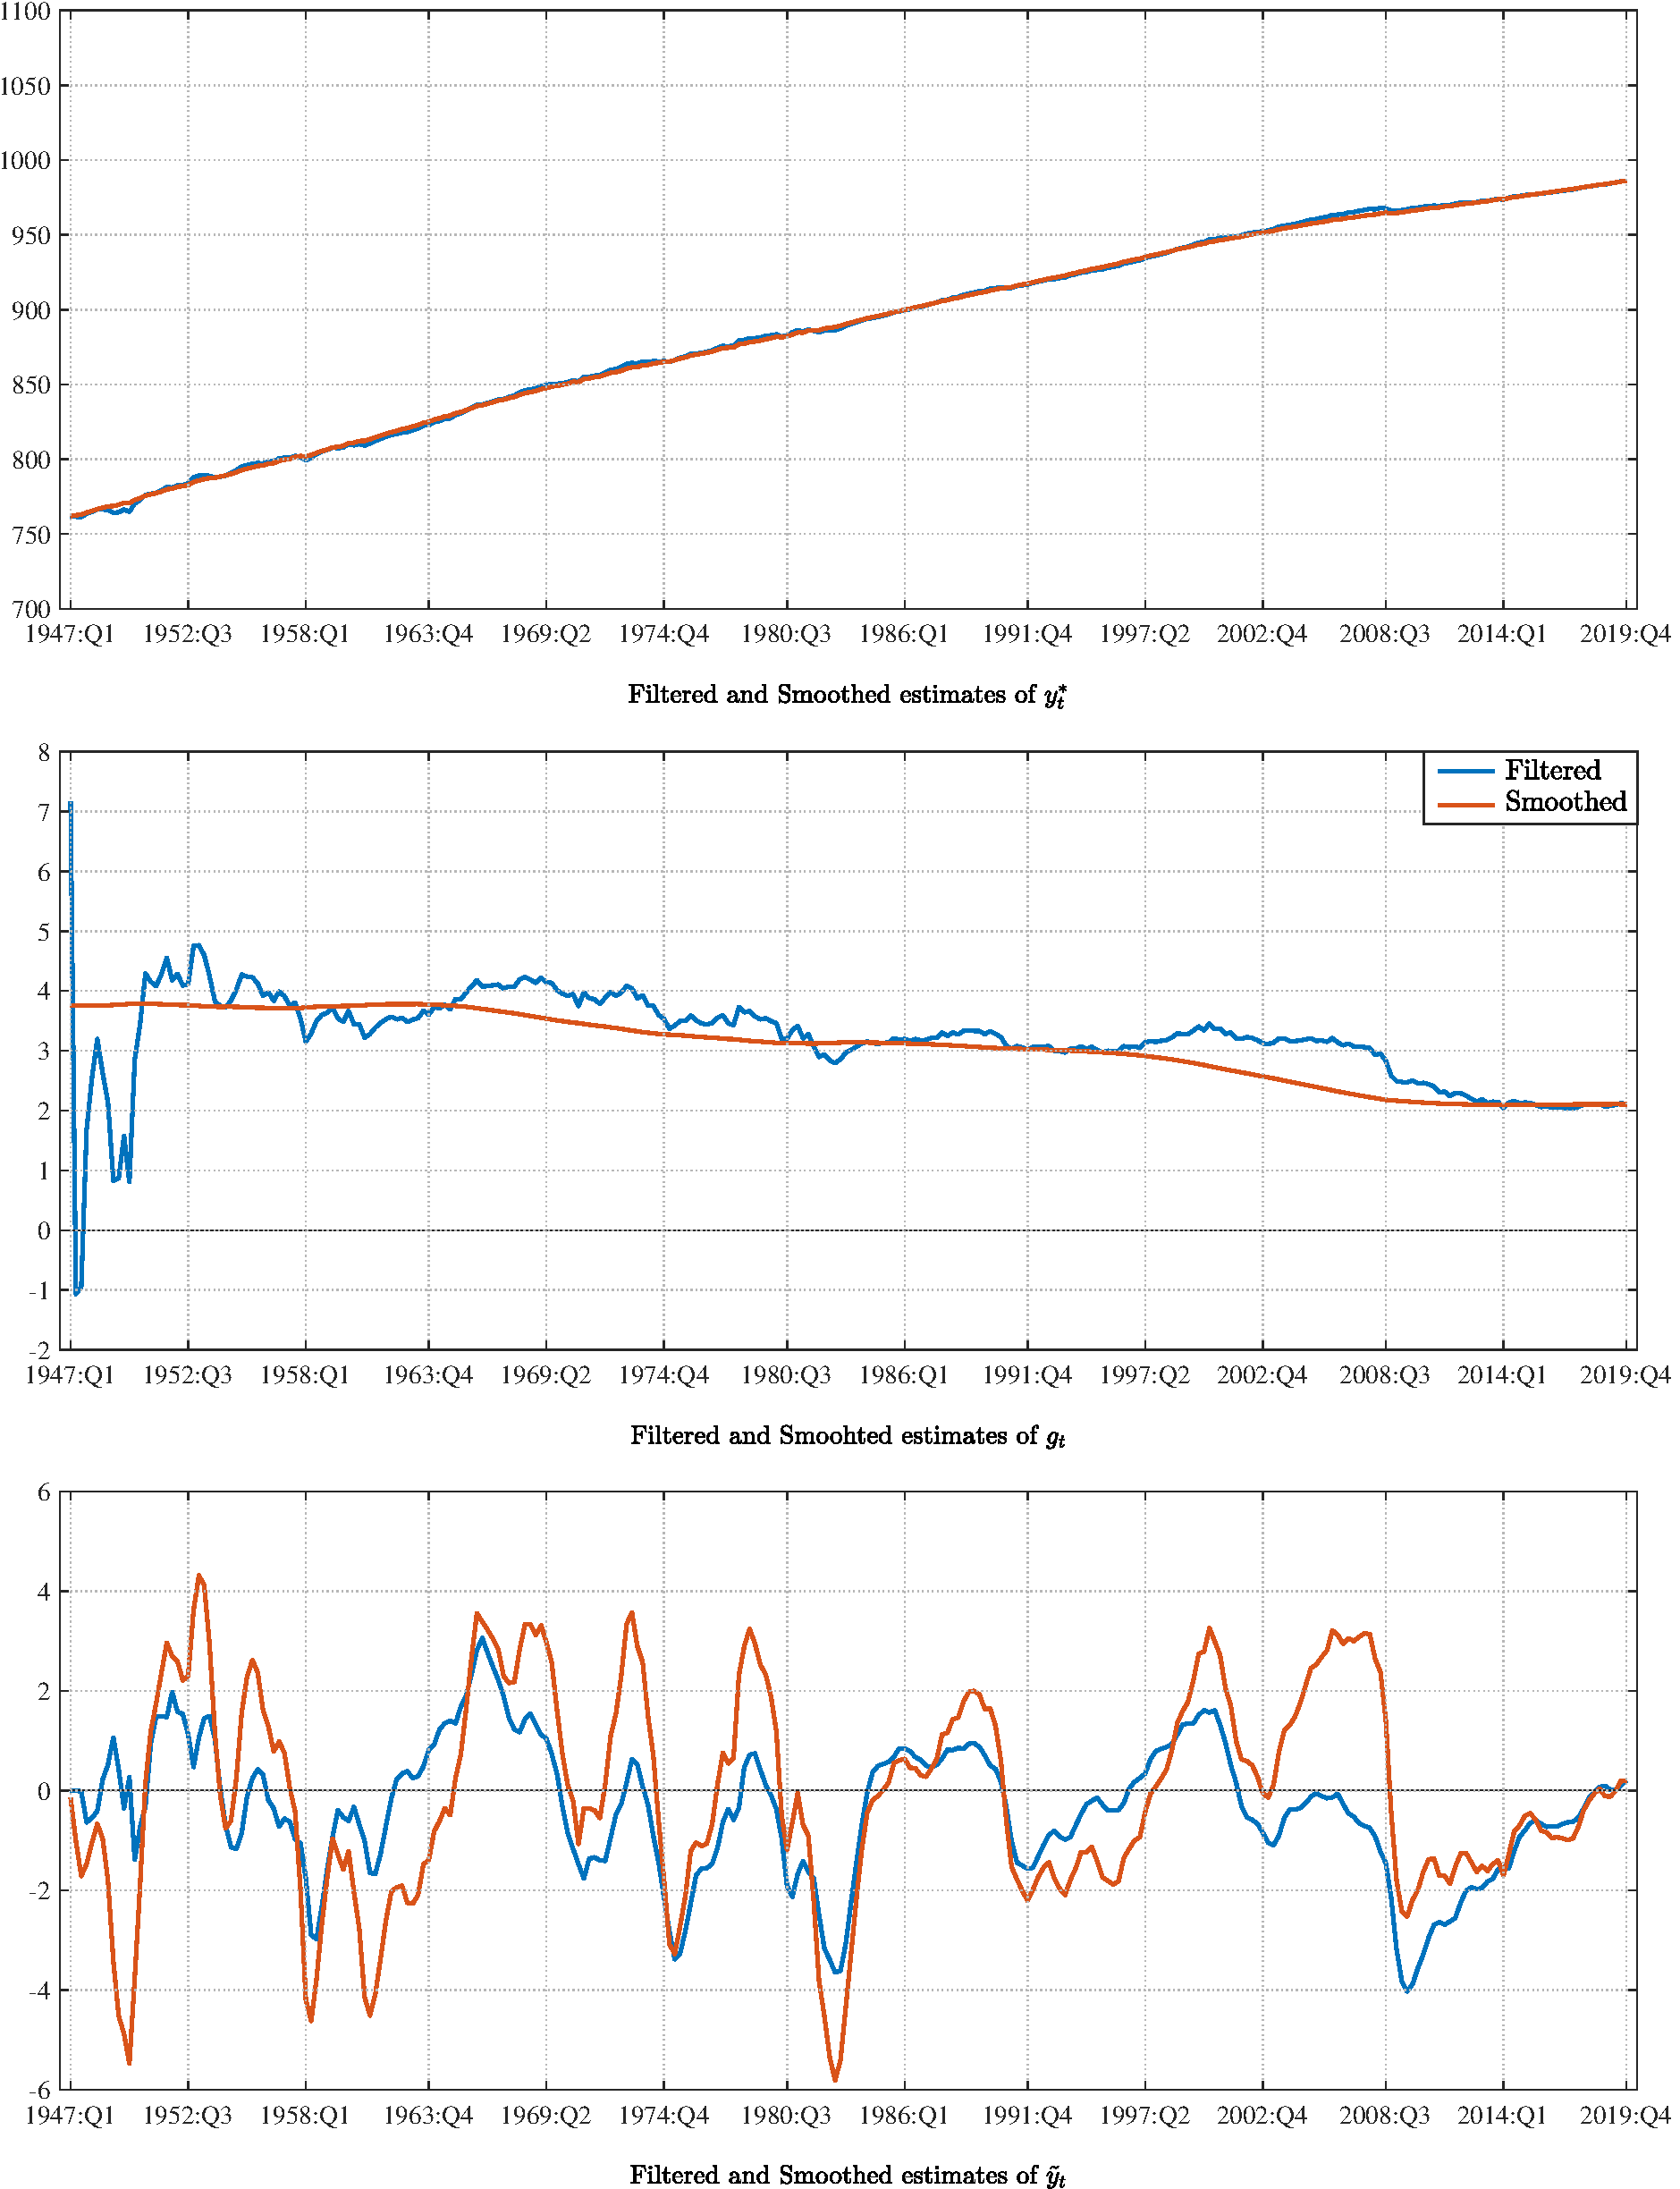
\includegraphics[angle=00, width=1\textwidth,trim={0 0 0 0},clip]{Clark_SSM} 
\vspace*{-2.5mm}
\caption{Filtered and Smoothed estimates trend, trend growth and cycle.}
\label{fig:KFS}
\end{figure}

\end{document}
